 \documentclass[12pt]{article}

\usepackage{epsfig}
\usepackage{comment}
\usepackage{natbib}
\usepackage{natbibmnfix}
\usepackage{graphicx}
\usepackage{color}
\usepackage{subfig}
\usepackage{bmpsize}
\usepackage{caption}
\usepackage{amsmath}
\usepackage{breqn}
\usepackage{wrapfig}
\usepackage{lipsum}
\usepackage{float}
%\usepackage{newcaptions} % changes the appearance of captions
\usepackage{url}
\usepackage{soul} % enables a better version of "\underline{}", called '\ul{}", which for instance permits linebreaks

\setul{1.5pt}{.4pt}
\newcommand{\UL}[1]{\ul{#1}}


\newcounter{dummy}
\def\@biblabel#1{\hspace*{\labelsep}[#1]}

\newcommand{\df}{\delta_{\rm F}}
\newcommand\atf{ATF}
\newcommand\scott[1]{\textcolor{blue}{\textbf{[Scott:}~#1} ]}

\def\lya{Ly$\alpha$}
\def\lyb{Ly$\beta$}
\def\etal{{\rm et~al.\ }}
\def\hmpc{\;h^{-1}{\rm Mpc}}
\def\hgpc{\;h^{-1}{\rm Gpc}}
\def\hkpc{h^{-1}{\rm kpc}}
\def\kpc{{\rm kpc}}
\def\kms{{\rm \;km\;s^{-1}}}
\def\shear{\langle \gamma^{2} (\theta) \rangle}
\newcommand{\phiv}{\mbox{\boldmath$\phi$}}
\newcommand{\thetav}{\mbox{\boldmath$\theta$}}
\def\pef{\par\noindent\hangindent 15pt}
\def\simlt{\lower.5ex\hbox{$\; \buildrel < \over \sim \;$}}
\def\lesssim{\lower.5ex\hbox{$\; \buildrel < \over \sim \;$}}
\def\simgt{\lower.5ex\hbox{$\; \buildrel > \over \sim \;$}}
\def\apj{{\it Astrophys. J.}}
\def\jcap{{\it  J. Cosmo. \& Astroparticle Phys.}}
\def\aj{{\it Astron. J.}}
\def\mnras{{\it Mon. Not. R. astr. Soc.}}
\newcommand{\apjl}{ApJL}
\newcommand{\nat}{Nature}
\newcommand{\araa}{ARA\&A}
\newcommand{\apjs}{ApJS}
\newcommand{\aap}{A\&A}
\newcommand{\pasp}{PASP}
\newcommand{\sfig}[2]{
\begin{center}
\includegraphics[width=#2]{#1}
\end{center}
        }
\newcommand{\Sjpg}[2]{
    \begin{figure}[htb]
    \sfig{./#1.jpg}{.9\columnwidth}
    \caption{{\small #2}}
    \label{fig:#1}
    \end{figure}
}
\newcommand{\Sfig}[2]{
    \begin{figure}[htb]
    \sfig{./#1.pdf}{.9\columnwidth}
    \caption{{\small #2}}
    \label{fig:#1}
    \end{figure}
}
\newcommand{\Spng}[2]{
    \begin{figure}[htb]
    \sfig{#1.png}{.9\columnwidth}
    \caption{{\small #2}}
    \label{fig:#1}
    \end{figure}
}

\newcommand{\Sfigtwo}[3]{
        \begin{figure}[htbp]
\sfig{#1.eps}{.3\columnwidth}
\sfig{#2.eps}{.3\columnwidth}
\caption{{\small #3}}
\label{fig:#1}
\end{figure}
}
\newcommand\be{\begin{equation}}
\newcommand{\Rf}[1]{\ref{fig:#1}}
\newcommand{\rf}[1]{\ref{fig:#1}}
\def\ee{\end{equation}}
\def\bea{\begin{eqnarray}}
\def\eea{\end{eqnarray}}
\newcommand{\vs}{\nonumber\\}
\newcommand{\ec}[1]{Eq.~(\ref{eq:#1})}
\newcommand{\Ec}[1]{(\ref{eq:#1})}
\newcommand{\eql}[1]{\label{eq:#1}}
\newcommand\cov{{\rm Cov}}
\newcommand\cl{{\mathcal{C}_l}}
\usepackage[margin=3.0cm]{geometry}
\usepackage{pslatex}
\newcommand\fnl{f_{\rm NL}}
\newcommand{\wh}[1]{\textcolor{blue}{[#1]}}
\newcommand{\tred}[1]{\textcolor{red}{[#1]}}

\newcommand\cp{C^{pri}}
\newcommand\ci{C^{ISW}}
\newcommand\cg{C^{gg}}
\newcommand\cgt{C^{g-ISW}}
\newcommand\tob{T^{\rm obs}}
\newcommand\aob{a^{\rm obs}}
\newcommand\tisw{T^{\rm ISW}}
\newcommand\aisw{a^{\rm ISW}}
\newcommand\si{C^{\rm ISW}_l}
\newcommand\sig[1]{C^{\rm g_{#1}-ISW}_l}
\newcommand\sg[2]{C^{\rm g_{#1}g_{#2}}_l}
\newcommand\tp{T^p}


%
% definitions
%
% A useful Journal macro
\def\Journal#1#2#3#4{{#1} {\bf #2}, #3 (#4)}
% Some useful journal names
\def\NCA{\em Nuovo Cimento\ }
\def\NPB{{\em Nucl. Phys.} B\ }
\def\PLB{{\em Phys. Lett.}  B\ }
\def\PRL{{\em Phys. Rev. Lett.\ }}
\def\PRD{{\em Phys. Rev.} D\ }
\def\prd{{\em Phys. Rev.} D\ }
\def\ZPC{{\em Z. Phys.} C\ }
\def\apj{{\em Ap. J.\ }}
\def\apjl{{\em Ap. J. Lett.\ }}
\def\la{\hbox{${_{\displaystyle<}\atop^{\displaystyle\sim}}$}}
\def\ga{\hbox{${_{\displaystyle>}\atop^{\displaystyle\sim}}$}}



\baselineskip=11pt
\def\msun{{\rm M_{\odot}}}

%\textheight=24.3cm
%\textwidth=16.8cm

\begin{document}
\topmargin=-2.105cm
\oddsidemargin=-0.1cm
\evensidemargin=0cm

\begin{center}
{\bf Extracting Information from the Large Scale Structure of the Universe\\}
Scott Dodelson (PI), Peikai Li, Andresa Rodrigues de Campos, John Urbanic, Tianke Zuang
\end{center}

\begin{small}


\section*{Summary} We request a total of 1M SU's on bridges for work analyzing data from the Dark Energy Survey and from large N-Body simulations.

\section{Introduction and Scientific Background}

Discoveries are hidden in previously unexplored domains. In the field of cosmology~\cite{Dodelson:2003ft}, the last unexplored domain is structure on the largest scales in the universe. Our ventures in this area to date have revealed the need for a mysterious substance dubbed dark energy that is driving the current epoch of acceleration of the universe and the need for dark matter unrelated to any particles that comprise us and the world around us. And there is more: there are hints of anomalies on the largest scales that may be related to yet new pieces of physics. 

We are fortunate to be living in a time when large surveys are capturing more and more parts of the sky. The Dark Energy Survey, for which the PI is the Co-Chair of the Science Committee, has surveyed one tenth of the sky out to redshifts $z>1$ (corresponding to distances billions of light years away when the universe was 8 billion years younger). The Large Synoptic Survey Telescope (LSST) will survey half of the sky every night and peer much deeper over its ten years of operations scheduled to begin in 2022. 

At the same time, numerical simulations have improved so that even their data cannot be analyzed on local machines. Analysis on simulations of course is a prerequisite for any robust analysis on real data. As a result, state of the art analyses of surveys takes place at national computational centers.

Our group is well-situated to make discoveries in this field because we can contribute:
\begin{itemize}
\item Leadership in current surveys
\item Theoretical expertise
\item Software Development
\item Resources at the PSC
\end{itemize} 
The PI led the effort to extract cosmology from DES using its first year of data, with fifteen papers submitted in 2017~(\cite{Abbott:2017wau} and references therein). There is a similar, although larger scale, effort ongoing right now to analyze three times as much data, the largest cosmological data set of its kind ever explored. Our leadership in this endeavor is the backbone of this proposal and drives many of the requirements and requests. We feel it is an opportunity for CMU and PSC to partner and be recognized for cutting edge work in cosmology. This will lay the groundwork for both institutions to continue their leadership during the next decade, the era of LSST.

Besides our leadership in surveys, we have presented a number of innovative ideas for extracting information from surveys and indeed are funded by both the NSF and DOE to apply these ideas to simulations and surveys. Exploring these new ideas on simulations is the second main thrust of this proposal. Here, too, our long term goal is to partner with PSC to become established leaders in the field of large survey analysis. As these ideas become generally accepted, we will be in an excellent position to implement them on DES and LSST.
\newcommand\cosmosis{{\tt cosmosis}}

Finally, we led the development of {\tt cosmosis}~\cite{Zuntz:2014csq}, a software framework designed for cosmological analyses. A large part of our request is to run Markov Chain Monte Carlo (MCMC) simulations (as we did for the Year 1 results) on DES data and simulations. This is a very low-risk high-reward program, as we are very familiar with the code base, and there is little development required. With the help of John Urbanic sitting in the Physics Department, we have been able to set up \cosmosis\ on several platforms and optimize it on bridges.

The goal of this proposal is to obtain the computational resources necessary to implement this program.

Here we briefly outline the scope of the two main thrusts of this proposal, relegating details to later sections. First, we aim to contribute heavily to the DES Year 3 (Y3) analysis (the first three years of data survey 5000 square degrees of the Southern Sky). DES is an international collaboration with over 500 members. The key project for Y3 will result in close to 30 papers culminating in the key paper that will be alphabetically ordered. 
Student Andresa Rodrigues de Campos is leading one of the {\it essential papers} that will feed into the key paper. Her work on exploring tension metrics will be the basis of making a quantitative decision about the compatibility of the universe recently as measured by DES with the very early universe as measured by experiments that probe the cosmic microwave background.

The second thrust is to explore the idea of inferring information about the largest wavelength perturbations in the universe by measuring small wavelength modes, exploiting the fact that the small-scale structure depends in a predictable way on the presence of long wavelength modes.



\section{Progress to Date and Motivation for Future Work}




\subsection{DES Chains}

In the results of the first year (Y1) of observations of The Dark Energy Survey (DES) \cite{Abbott:2017wau}, we combined data from galaxy clustering~\cite{Elvin-Poole:2017xsf}, cosmic shear~\cite{Troxel:2017xyo} and their cross-correlation, galaxy-galaxy lensing~\cite{Prat:2017goa}. The first of these is the traditional way of inferring information about the mass of the universe using astronomical surveys: assume that galaxies trace mass, measure the statistics of the galaxy distribution, and compare with the theoretical predictions for these statistics, again assuming that the galaxy statistics that are measured are related to the mass statistics that are theoretically predicted. The assumed relation is called \emph{bias}. The second observable measured was \emph{cosmic shear}, the correlation between the shapes of background galaxies. These are distorted by the intervening mass distribution, so cosmic shear offers a unique way to probe the mass distribution in the universe without assuming anything about bias. These two sets of statistics are supplemented by one that cross-correlates the two: the positions of the foreground galaxies with the shapes of background galaxies. In each case, the two-point function is measured and computed theoretically using \cosmosis. 


The predictions depend on 26 different parameters, six that determine the cosmology and twenty other so-called ``nuisance'' parameters that are needed to quantify various astrophysical uncertainties. For example, nine parameters are needed to capture the uncertainty in how far away from us are all the galaxies used in the analysis. Computing the likelihood in this 26-dimensional space requires clever sampling techniques. For Y1, we used the {\tt multinest} sampler~\cite{Feroz:2008xx} running on the midway computing cluster at the University of Chicago. Each run took of order one day of clock time depending on the data sets used. Using 128 cores, this corresponds to between 1000-5000 CPU hours per run. In total, we used 1 million CPU hours for the Y1 analysis, corresponding to a few hundred runs. 

One of the most important goals of DES is to determine the consistency of what has become the concordance model of cosmology, so-called $\Lambda$CDM. This model is built on the assumption that the dark energy that contributes 70\% of the energy in the universe is a cosmological constant (the Greek letter $\Lambda$) with a value that is extraordinarily difficult to reconcile with our theoretical prejudices. As such, a large thrust is to stress-test $\Lambda$CDM. DES can do this by measuring some of the same parameters within $\Lambda$CDM that have already been pinned down precisely by another set of experiments, those that probe the universe at very early times, when the universe was only 400,000 years old. If the DES measurements are found to be inconsistent with the early-time measurements (cosmic microwave background or CMB), then $\Lambda$CDM will need to be replaced.

%
% (3x2-point correlations), and showed the potential power of combining these different cosmological probes to constrain cosmology. Recently, we took this approach one step further by combining these data also with Type Ia supernova lightcurves and the baryon acoustic oscillation feature, both also measured by DES \cite{Abbott:2018wzc}. From this multi-probe approach, we are able to rule out a Universe with no dark energy using data only from DES. 

%Currently, several large photometric surveys are capable of independently combining multiple cosmic probes and, over the following decade, new generation surveys, such as the  Large  Synoptic  Survey  Telescope (LSST), will provide powerful constraints on the distance-redshift relation and the growth of structure. The union of these results is expected to have huge constraining power, being able to provide us with the necessary insights to understand nature of dark energy.

Clearly then, one crucial aspect of this approach is the ability to evaluate whether all data being used together is consistent, i.e. is there tension between the datasets. A tension metric should be robust enough to assess the compatibility of both different probes from a single experiment and data from different experiments. This is especially relevant in the case in which the experiments being combined are measuring very different features, e.g. the Cosmic Microwave Background (CMB) measures properties of the Universe only  $400,000$  years after the  Big  Bang, while photometric surveys measure the Large Scale Structure (LSS) of the Universe after dark energy has already dominated.

For Y1, the metric we used was Bayesian evidence~\cite{Marshall:2003ez}. Since then, several groups have criticized this metric as being overly sensitive to priors~\cite{Raveri:2018wln,Handley:2019wlz}. Therefore, an important part of the DES-Y3 analysis is to test different tension metrics on simulated data, where we know the internal tension before the analysis. %So far, we have simulated DES data sets and are using them to quantify how well metrics commonly used for measuring concordance and discordance between datasets, e.g. Bayesian Evidence Ratio, can identify tensions between the CMB and DES. 
In order to evaluate tension metrics in terms of the values of cosmological parameters, we generated a set of simulated DES data-vectors. One of these data-vectors was built to have exactly the same cosmology as the one recovered from CMB data, while the others contain $1\sigma$ to $5\sigma$ shifts in the two main parameters measured by DES, the total matter density, $\Omega_m$, and the amplitude of the matter power spectrum at a scale of $8h^{-1}$Mpc, $\sigma_8$. By knowing the amount of tension each one of these data-vectors contain with respect to the CMB-preferred cosmology, we are able to quantify the performance of different tension metrics.



\subsection{Anisotropic Clustering on Simulations}
Gravity acts to bring matter together since it is an attractive force. Early on in the history of the universe, all regions contained very similar amounts of matter with only small perturbations. Over billions of years, though, those small perturbations grew via gravitational instability so that the universe has become inhomogeneous. Inhomogeneities are quantified via
\be
\delta(\vec x) \equiv \frac{\rho(\vec x) - \bar\rho}{\bar\rho}.\ee
This dimensionless over-density begins much less than one everywhere and gradually grows to become very non-uniform, with values ranging from $-1$ up to $10^{30}$ or even larger. This evolution to nonlinearity can be studied, on large scales, using perturbation theory in Fourier space.

\Spng{nbody}{The ratio of long wavelength modes inferred from the quadratic estimator of \ec{quad} to the actual values of these modes. In both cases, we use the same catalog from an N-Body simulation. The fairly sharp peak indicates that the estimator has large signal to noise. The fact that the peak is at a ratio of 2 instead of one indicates that more care must be taken relating items in the catalog to mass. For that purpose, we need to access the raw data from the simulation, which can be done only with the computing power requested in this proposal.}


Perturbation theory makes an interesting prediction about the first-order correction to linear evolution. For a short wavelength mode $\delta(\vec{k}_s)$, this first nonlinear contribution can be shown to be~\cite{Bernardeau:2001qr} equal to 
\begin{eqnarray}
\delta^{(2)}(\vec{k}_s)=\int\frac{d^{3}\vec{k}_l}{(2 \pi)^3}F_2(\vec{k}_s-\vec{k}_l,\vec{k}_l)\delta_{s}^{(1)}(\vec{k}_s-\vec{k}_l)\delta_l^{(1)}(\vec{k}_l)\eql{pert}
\end{eqnarray}
where the upper-subscript means the order of perturbation theory and $F_2$ is a known function of its arguments. Note that the second order contribution to the small wavelength modes are determined by a convolution of the product of a small and large wavelength mode. 
This arises physically because small structure structure varies depending on the large scale environment in which it resides. \ec{pert} has the exact same form as the impact that the gravitational field has on the temperature field of the CMB, an effect called \emph{CMB lensing}. That effect has been exploited and measured by forming \emph{quadratic estimators} of the temperature fields to infer the large scale modes of the gravitational field responsible for the lensing~\cite{Hu:2001tn}.
Similar to the CMB lensing case, we can construct a quadratic estimator in this case:
\begin{eqnarray}
\hat{\delta}_l^{(1)}(\vec{k}_l)=A(\vec{k}_l)\int \frac{d^3 \vec{k}_s}{(2\pi)^3} g(\vec{k}_s,\vec{k}_s')\delta_s(\vec{k}_s)\delta_s(\vec{k}_s')\eql{quad}
\end{eqnarray}
with $g$ being a weighting function, $\vec{k}_s'=\vec{k}_l-\vec{k}_s$ and $A$ is defined to require that the expectation value of the estimator $\langle \hat{\delta}_l^{(1)}(\vec{k}_l) \rangle=\hat{\delta}_l^{(1)}(\vec{k}_l)$, the actual long wavelength mode. These functions then are determined to be:
\begin{eqnarray}
A(\vec{k}_l)&=&\bigg[\int \frac{d^3 \vec{k}_s}{(2\pi)^3} g(\vec{k}_s,\vec{k}_s')f(\vec{k}_s,\vec{k}_s')  \bigg]^{-1} \\
f(\vec{k}_s,\vec{k}_s')&=&F_2(-\vec{k}_s,\vec{k}_s+\vec{k}_s')P(k_s)+F_2(-\vec{k}_s',\vec{k}_s+\vec{k}_s')P(k_s') \\
g(\vec{k}_{s_1},\vec{k}_{s_1}')&=&\frac{f(\vec{k}_{s_1},\vec{k}_{s_1}')}{2P(k_{s_1})P(k_{s_1}')}
\end{eqnarray}
where $P(k)$ is the linear power spectrum of matter.
%And $F_2$ is a known function with pre-determined mathematical expression. 

\ec{quad} is remarkable in that it empowers us to learn about the universe on large scales by measuring perturbations on small scales. 
The goal of our project is to use data from N-Body simulations, which captures all nonlinear effects, and compute the value of the quadratic estimator from it. After comparison to direct data from the N-Body simulation, we can further determine if this hypothesis is correct and can be applied to surveys.


To date, we have been limited by computational power. On our laptop, we used a catalog produced by Rockstar Halo~\cite{2013ApJ...762..109B} finder based on an underlying N-Body simulation. The results are shown in Fig.~\rf{nbody}. While the signal to noise is apparently quite large, there is a factor of 2 difference between the estimated modes and their true values. This is very likely due to our assumption that the catalog objects have uniform mass. It is imperative therefore that we analyze the raw N-Body data itself.
%So we want to try with mass particle position data instead of Halo position data and see if it works. \\


\section{Proposed Computational Methods}
\subsection{DES Chains}

The {\tt cosmosis} framework has all the resources necessary for the analysis we are going to perform. We have already used it to extract the preferred cosmology from the Planck 2015 likelihood  by sampling it using {\tt multinest}. From this run we inferred the value of the cosmological parameters that best-fit the $\Lambda$CDM model according to Planck data and used these values to generate a baseline simulated DES-like data-vector, see Figure \ref{figure1}.


The simulated data is composed by galaxy clustering, cosmic shear and galaxy-galaxy lensing information just like it would be measured by DES, and it was also generated using {\tt cosmosis}. Besides the baseline data-vector, we also generated data in which the cosmological parameters $\Omega_m$ and $\sigma_8$ are shifted with respect to their "true" value, introducing a known tension between the Planck data and the simulated shifted data. For each parameter, we generate five data-vectors in which the corresponding parameter is shifted from its baseline value from $1\sigma$ to $5\sigma$. This choice is due to the fact $\sigma$s are a standard measure of agreement level, which means that if we use a tension metric to compare two data sets which have parameters that disagree by more than $3\sigma$, the tension metric should be flagging this disagreement. 

%We used the {\tt cosmosis} framework to run the Planck 2015 likelihood and get the value of the cosmological parameters that best-fit the $\Lambda$CDM model according to Planck data. This cosmology was used to generate a baseline simulated data-vector, corresponding to a 3x2pt DES data-vector, containing the galaxy clustering, cosmic shear and galaxy-galaxy lensing information that would be measured by DES, but with the cosmology ensured to be the same as the one measured by Planck, such that the two experiments completely agree, see Figure \ref{figure1}. Then, we generated simulated data-vectors with $1\sigma$ to $5\sigma$ shifts in $\Omega_m$ and $\sigma_8$ parameters. 

\begin{figure}[h!]
\begin{center}
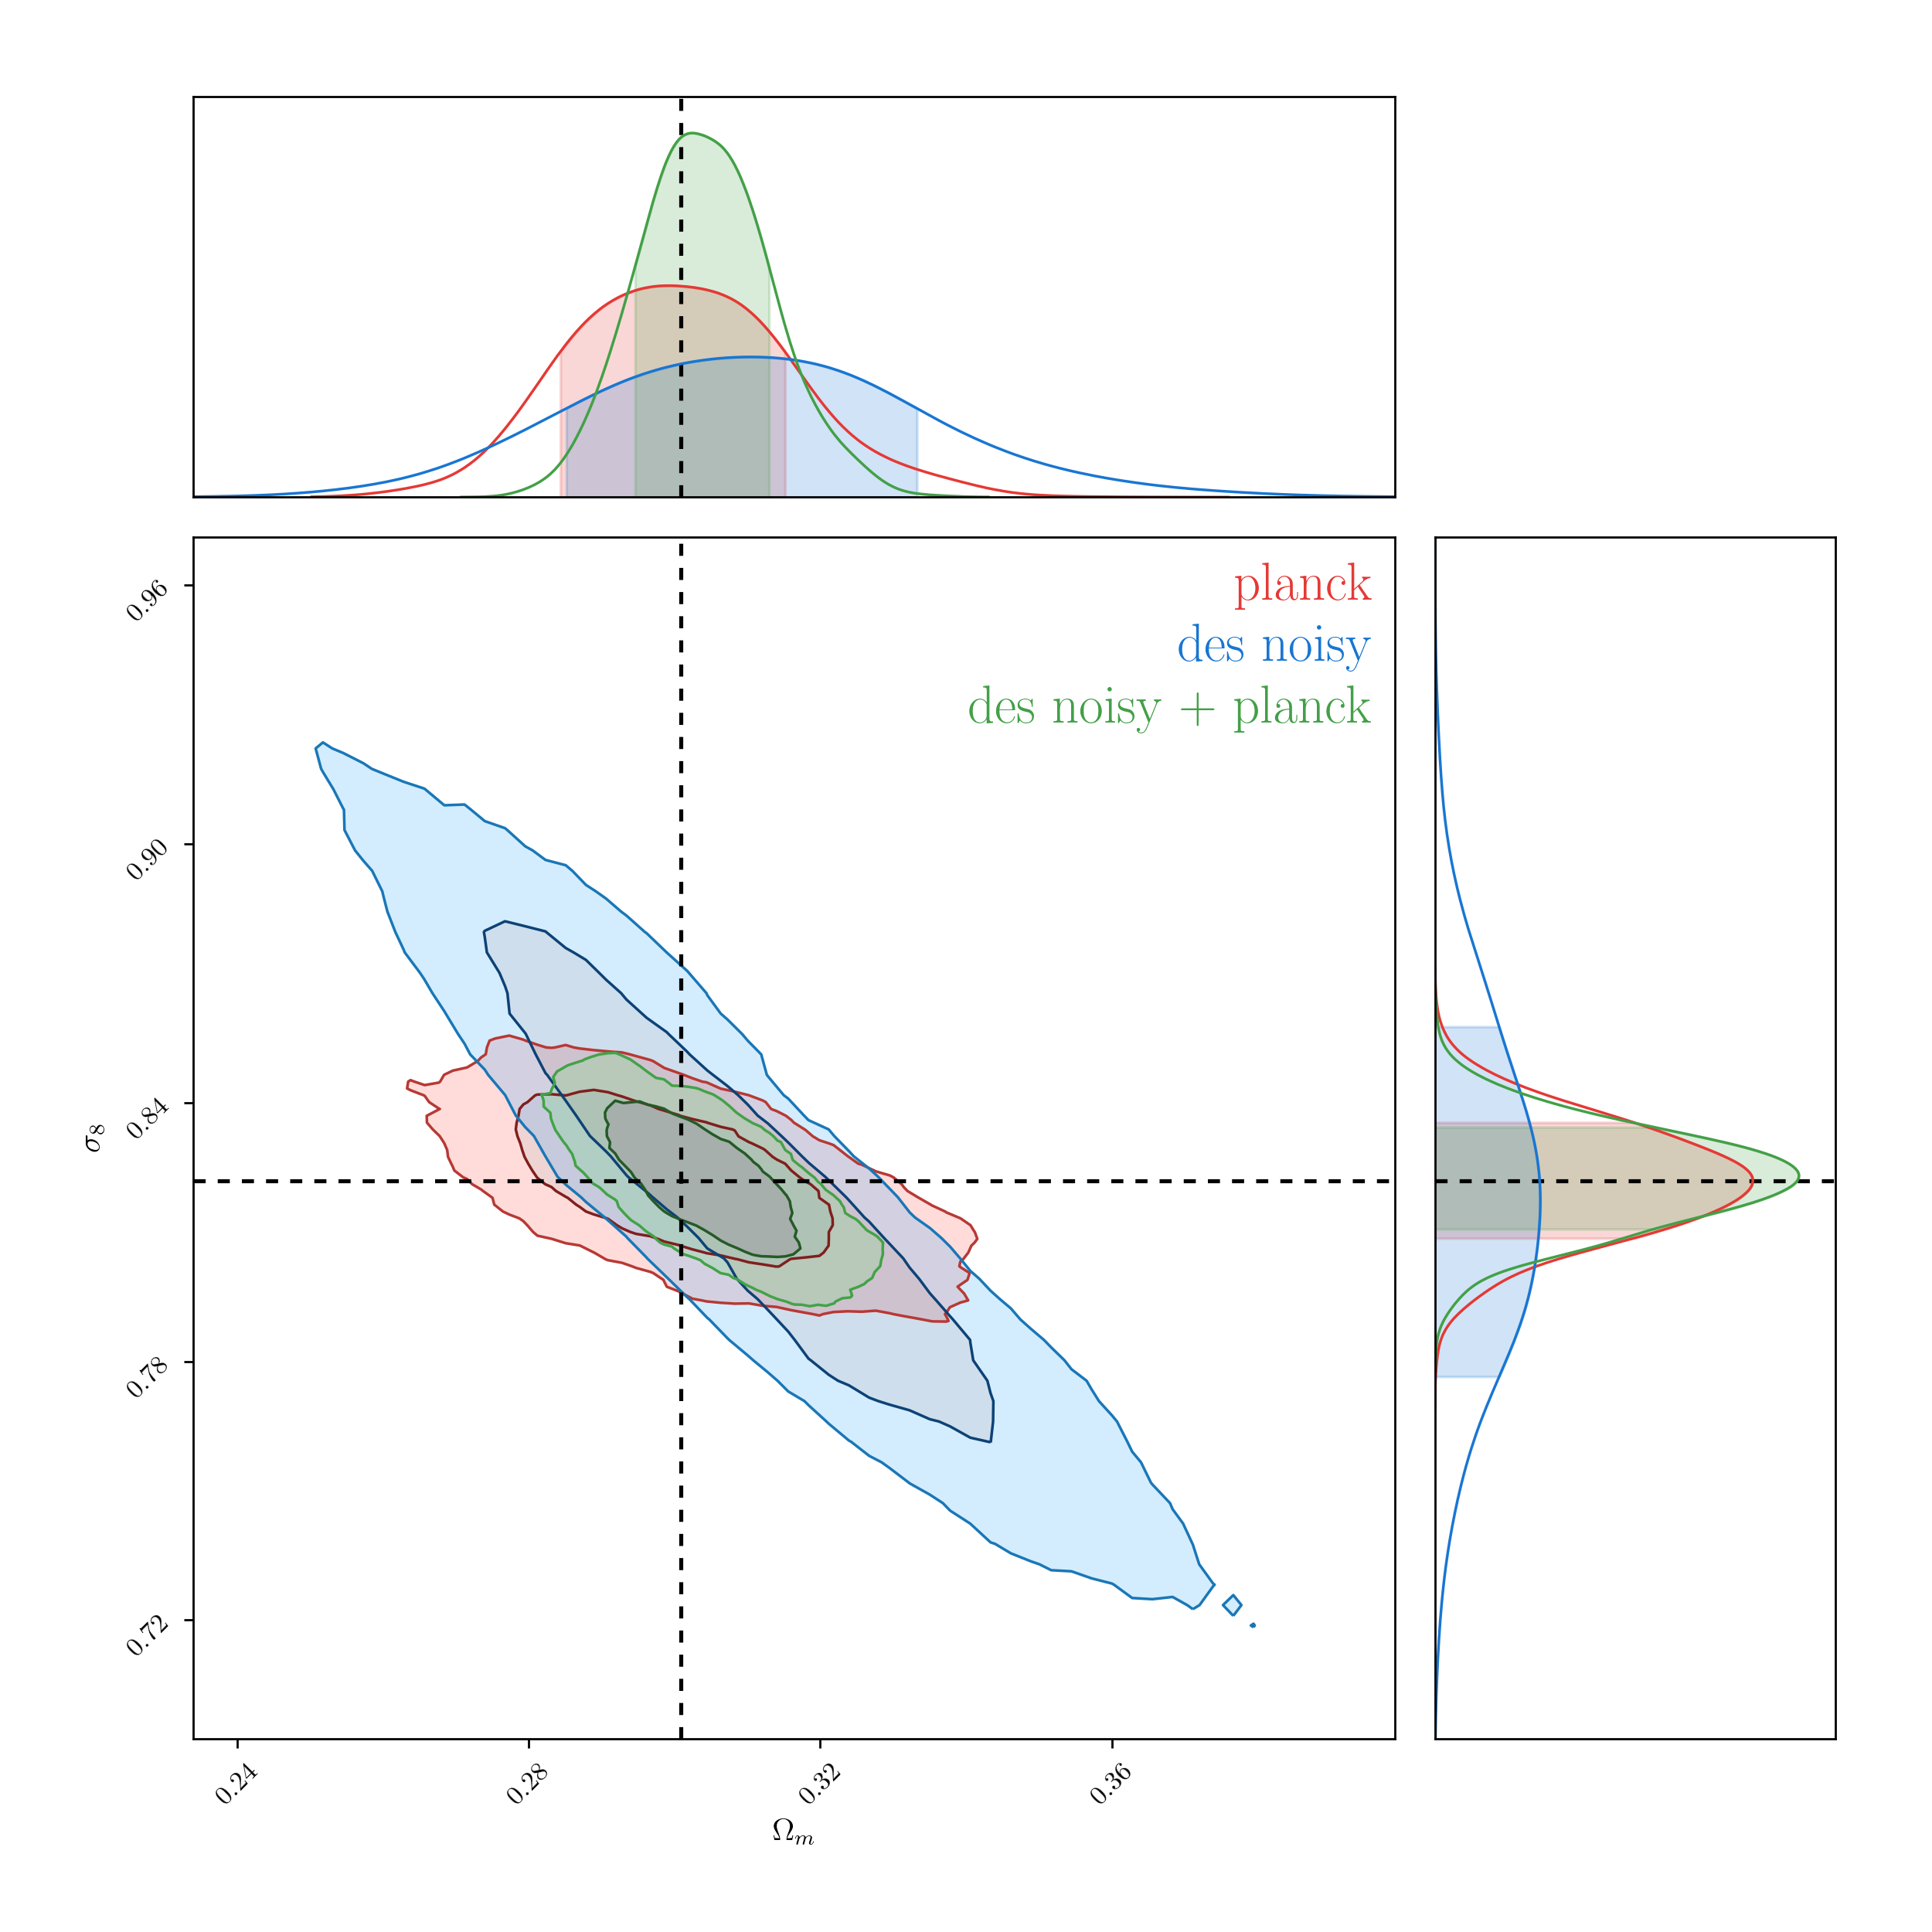
\includegraphics[height=12cm]{des+planck_poly2D.png}
\end{center}
 \caption{Posterior of Planck likelihood, red, DES 3x2pt simulated data, blue, and the combination of Planck and DES, green.}
\label{figure1}
\end{figure}

The next step is run these simulated data-vectors in combination with the Planck likelihood to perform the combined DES+Planck analysis. There are a total of 10 chains to be run in order to finalize the project which investigate the performance of the tension metrics, and each of these runs take of order 120 hours using 128 cores, corresponding to approximately 15,000 CPU hours per run.

%We are on the stage in which these simulated data-vectors then need to be run through the DES 3x2pt pipeline and through the combined DES+Planck pipeline to obtain the posterior and estimate the evidence in each case. 

\subsection{Anisotropic Clustering on Simulations}
We would like to download and read N-Body simulation data from \url{https://www.cosmosim.org}; precisely, we will need to use positions of approximately $1/100$ particles from HugeMDPL simulation at a snapshot of redshift $z=0$, which is a N-Body simulation with Planck cosmology, box size $4000 \, \rm  Mpc/h$ and $4096^3$ particles in total. Our main goal is to download part of the data we need from this website and save to our own text format. We will simply use readgadget function from python package to read these files and extract useful data we need. Then we will do a Fast Fourier Transform into a mesh with $1280^3$ cells, so we require full disk and memory.\\
The overall data of snapshot $z=0$ has a size of $1.7$ Tb. The Leibniz-Institute for Astrophysics Potsdam in collaboration with the MultiDark consortium created the MultiDark Database including HugeMDPL. Format of the files is gadget binary file. \\
We will use $wget$ to download these files. I am a registered user of \url{https://www.cosmosim.org} so I have the permission to download these data, and if we can form a paper out of these data, we will cite~\cite{Klypin:2016kl} and give credits to this database.


\section{Proposed Analyses and Justification of Requested Resources}

The analyses described in the previous sections can be summarized as:
\begin{enumerate}
\item MCMC chains for the DES-Y3 tensions paper
\item MCMC chains for the DES-Y3 data, key project paper
\item Quadratic estimator applied to large N-Body simulations
\end{enumerate}
The first two of these will be an integral part of the DES Year 3 data and science release, within the next six months. The last will lead to a paper or two over the same time scale and then -- if successful -- forge the way for analyses on real data.

The most time consuming chains for both 1 and 2 are those that analyze several data sets, especially Planck and DES. These chains can require up to 30,000 CPU hours. For 1, we must run at least ten of them (one for each of the ten simulated data sets shifted by x$sigma$ in one of two parameters). For 2, we expect to run about twice that many, accounting for different cosmological models that need to be run and different combinations of data sets (e.g., DES+Planck, DES lensing only+Planck, DES+non-CMB external experiment, $\ldots$). Therefore, we are hoping that 1M SU's will be sufficient; indeed, this is what the PI ran through at Chicago for the Y1 analysis.

The third project requires much CPU hours, but disk space beyond the range of local machines and memory to store and analyze the simulations.


\begin{table}[h!]
\begin{center}
%\setlength{\extrarowheight}{7pt}
  %\resizebox{\columnwidth}{!}{
\begin{tabular}{c|cc|c}
%\hline
 Chain         & $\#$ Cores &  Time & CPU-hours   \\ 
\hline
%\hline
%Baseline & $7.72$ & Strong Consistence & $0.81$ \\ 
DES only baseline & $128$ & $60$h & $7680$  \\  
DES + Planck baseline & $128$ & $120$h & $15360$  \\  
\hline
DES only $\sigma_8$ - $1\sigma$ & $128$ & $60$h & $7680$  \\ 
DES only $\sigma_8$ - $2\sigma$ & $128$ & $60$h & $7680$  \\ 
DES only $\sigma_8$ - $3\sigma$ & $128$ & $60$h & $7680$  \\ 
DES only $\sigma_8$ - $4\sigma$ & $128$ & $60$h & $7680$  \\ 
DES only $\sigma_8$ - $5\sigma$ & $128$ & $60$h & $7680$  \\   
DES only $\Omega_m$ - $1\sigma$ & $128$ & $60$h & $7680$  \\  
DES only $\Omega_m$ - $2\sigma$ & $128$ & $60$h & $7680$  \\ 
DES only $\Omega_m$ - $3\sigma$ & $128$ & $60$h & $7680$  \\   
DES only $\Omega_m$ - $4\sigma$ & $128$ & $60$h & $7680$  \\ 
DES only $\Omega_m$ - $5\sigma$ & $128$ & $60$h & $7680$  \\ 

\hline
DES + Planck  $\sigma_8$ - $1\sigma$ & $128$ & $120$h & $15360$  \\ 
DES + Planck  $\sigma_8$ - $2\sigma$ & $128$ & $120$h & $15360$  \\ 
DES + Planck  $\sigma_8$ - $3\sigma$ & $128$ & $120$h & $15360$  \\ 
DES + Planck  $\sigma_8$ - $4\sigma$ & $128$ & $120$h & $15360$  \\ 
DES + Planck  $\sigma_8$ - $5\sigma$ & $128$ & $120$h & $15360$  \\  
DES + Planck $\Omega_m$ - $1\sigma$ & $128$ & $120$h & $15360$  \\  
DES + Planck  $\Omega_m$ - $2\sigma$ & $128$ & $120$h & $15360$  \\ 
DES + Planck  $\Omega_m$ - $3\sigma$ & $128$ & $120$h & $15360$  \\   
DES + Planck  $\Omega_m$ - $4\sigma$ & $128$ & $120$h & $15360$  \\ 
DES + Planck  $\Omega_m$ - $5\sigma$ & $128$ & $120$h & $15360$  \\ 
\hline
 & &  & Total: \\ 
\end{tabular}
%}
\caption{Chains to be run. (needs to include the DES chains for the Y3KP )}
\label{tab:post}
\end{center}
\end{table}


\section{Computational Resources}

The Dark Energy Survey collaboration have access to computing time on NERSC. The total allocation is 30,000,000 CPU-hours for the use of the entire collaboration, with a  limit of 900,000 CPU-hours per user. So far, all the  progress that has been done in the tensions project was achieved running chains at NERSC, but keep using this machine for
completing this project is problematic due to two main reasons. First, the amount of CPU-hours that are still available for the student, approximately 50,000, is not enough to conclude the project . The second issue is the the long waiting time for the jobs to start. Since this resource is shared by the 400 collaboration members, the queue time for a job to start has been approximately 4 days. In principle, the tensions project must be concluded before the final analysis of Y3 data starts, since it will dictates how to perform it consistently, which implies we are very time constrained and need it to be concluded as soon as possible.



\section{Research Plan}

\section{Grant Support}

The PI is supported by the U.S. Dept. of Energy contract DE-SC0019248 for the project ``Physics from Cosmic Surveys.'' He is also co-I on the proposal ``New Vistas in Weak Lensing,'' funded by the NSF, tracking number 1909193. Both of these proposals fund all personnel required to successfully carry out the projects highlighted in this proposal.

\section{Total Allocation Request}

Our total request is:

{\bf 1,000,000 SUs on Bridges}

{\bf 10 PetaBtyes of storage}

\end{small}

%\newpage

\bibliographystyle{plain}
\bibliography{refs}

\end{document}
